\documentclass{beamer}

% packages
\usepackage{cancel}
\usepackage{mdframed}
\usepackage[T1]{fontenc}
\usepackage[utf8]{inputenc}
\usepackage{graphicx}
\usepackage{amsmath}
\usepackage{caption}            
\usepackage{subcaption} 
\usepackage[absolute,overlay]{textpos}
\usepackage{listings}
\usepackage{pifont}
\usepackage{booktabs}
\usepackage{siunitx}
\usepackage{amssymb}
\usepackage{tcolorbox}

% theme
\usetheme{AnnArbor}
\setbeamertemplate{navigation symbols}{}

% colours
\definecolor{green}{RGB}{0, 140, 69}
\definecolor{red}{RGB}{205, 33, 42}
\definecolor{NavyBlue}{RGB}{0,0,128}
\definecolor{RoyalBlue}{RGB}{65,105,225}
\definecolor{BabyBlue}{RGB}{137, 207, 240}
\definecolor{SkyBlue}{RGB}{135, 206, 250}
\definecolor{CornflowerBlue}{RGB}{100, 149, 237}
\setbeamercolor{palette primary}{bg=SkyBlue}
\setbeamercolor{palette secondary}{bg=CornflowerBlue}
\setbeamercolor{palette tertiary}{bg=RoyalBlue}
\setbeamercolor{frametitle}{bg=white}
\setbeamercolor{section in head/foot}{fg=white} 
\setbeamercolor{subsection in head/foot}{fg=white} 
\setbeamercolor{author in head/foot}{fg=white} 
\setbeamercolor{date in head/foot}{fg=white} 
\setbeamercolor{title in head/foot}{fg=white} 

% information
\title{PerfTuner}
\author{Alexander, Soumili, Thomas}
\date{20 March 2024}

\begin{document}

% title frame
\begin{frame}
    \begin{center}
        {\color{RoyalBlue}{\bf \LARGE PerfTuner}}

        \vspace*{0.5cm}
        
        {\color{SkyBlue}{\bf \Large \textit{- Vectorizing Programs by Exploiting LLMs -}}}

         \vspace*{1cm}

        {\color{RoyalBlue}{\bf \Huge Final Presentation}}

        \vfill

        {\color{gray}{\bf \large Alexander, Soumili, Thomas}}

        \vspace*{0.5cm}
         
         {\color{gray}{\bf \normalsize 20 March 2024}}
    \end{center}
\end{frame}

\begin{frame}{Best Results: Could All Problems Be Solved?}
    \begin{table}[htbp]
        \centering
        \begin{tabular}{@{}lc@{}}
            \toprule
            \textbf{Problem}                         & \textbf{solved?}\\ \midrule
            BitwiseAND                               & \textcolor{green}{\ding{51}}\\
            LinearCombination (2 versions)           & \textcolor{green}{\ding{51}}\\
            MatrixMultiplication (3 versions)        & \textcolor{green}{\ding{51}}\\
            MatrixVectorMultiplication               & \textcolor{green}{\ding{51}}\\
            ScalarMultiplication                     & \textcolor{green}{\ding{51}}\\
            Scalarproduct (3 versions)               & \textcolor{green}{\ding{51}}\\
            VectorAddition                           & \textcolor{green}{\ding{51}}\\
            BitwiseLogicCombined                     & \textcolor{green}{\ding{51}}\\
            LU1                                      & \textcolor{green}{\ding{51}}\\
            Transpose                                & \textcolor{green}{\ding{51}}\\
            LU3                                      & \textcolor{green}{\ding{51}}\\ 
            \bottomrule
        \end{tabular}
    \end{table}
    \vfill
    \centering
    \textcolor{orange}{\textbf{$\Rightarrow$ \textit{Eventually} we can solve everything}}
\end{frame}

\begin{frame}{Best Results: Could All Problems Be Solved \textit{Constantly}?}
    \begin{figure}
        \centering
        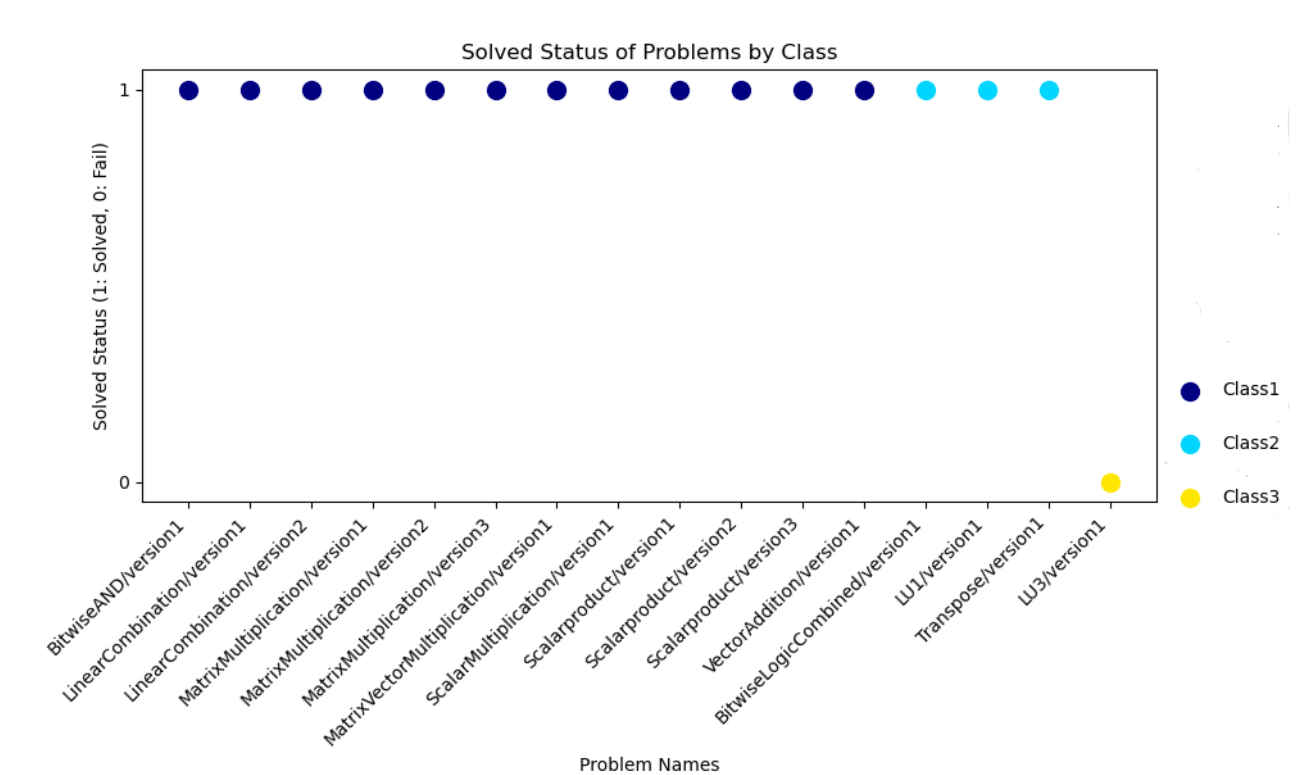
\includegraphics[height=0.8\textheight]{images/solved_status_graph.png}
    \end{figure}
\end{frame}

\begin{frame}{Finding the Snippet List: Meta-Strategies}
    \begin{figure}
        \centering
        \hspace*{0.5cm} 
        \begin{subfigure}[b]{0.25\textwidth}
            \centering
            
\includegraphics[width=0.9\textwidth]{images/voting.png}
            \caption{Voting}
        \end{subfigure}
        \hfill
        \begin{subfigure}[b]{0.25\textwidth}
            \centering
            
\includegraphics[width=0.9\textwidth]{images/tournament.png}
            \caption{Tournament}
        \end{subfigure}
        \hfill
        \begin{subfigure}[b]{0.25\textwidth}
            \centering
            
\includegraphics[width=0.9\textwidth]{images/default.png}
            \caption{Default}
        \end{subfigure}
        \hspace*{0.5cm} 
    \end{figure}
\end{frame}

\begin{frame}{Comparing the Meta-Strategies: Snippet, Quality, Success}
    \small
    \begin{table}[htbp]
        \centering
        \begin{tabular}{l|ccc|ccc|ccc}
            \toprule
            \textbf{Problem} & \multicolumn{3}{c|}{\textbf{Voting}} & \multicolumn{3}{c|}{\textbf{Tournament}} & \multicolumn{3}{c}{\textbf{Default}} \\
            \midrule
            BitwiseAND & 9 & \num{-2.1} & \num{0.2} & 5 & \num{-0.1} & \num{0.9} & 10 & \num{-1.2} & \num{0.2}\\
            LinearCombination & 9 & \num{-2.3} & \num{0.1} & 3 & \num{-1.3} & \num{0.3} & 10 & \num{-1.4}& \num{0.1} \\
            MatrixMult. & 9 & \num{-2.0} & \num{0.0} & 6 & \num{-2.0} & \num{0.0} & 10 & \num{-2.0} & \num{0.1}\\
            MatrixVectorMult. & 9 & \num{-2.1} & \num{0.0} & 3 & \num{-1.9} & \num{0.0} & 10 & \num{-1.9} & \num{0.1}\\
            ScalarMult. & 11 & \num{-1.4} & \num{0.2} & 3 & \num{-1.9} & \num{0.3} & 10 & \num{-0.7} & \num{0.5} \\
            Scalarproduct & 11 & \num{-1.4} & \num{0.1} & 3 & \num{-1.3} & \num{0.4} & 10 & \num{-1.9} & \num{0.1}\\
            VectorAddition & 9 & \num{-2.0} & \num{0.0} & 1 & \num{-0.8} & \num{0.4} & 10 & \num{-1.8} & \num{0.0}\\
            BitwiseLogicComb. & 9 & \num{-1.1} & \num{0.4} & 5 & \num{-1.5} & \num{0.2} & 10 & \num{-1.2} & \num{0.4} \\
            LU1 & 9 & \num{-2.0} & \num{0.0} & 10 & \num{-1.6} & \num{0.1} & 10 & \num{-2.1} & \num{0.0} \\
            Transpose & 9 & \num{-2.1} & \num{0.0} & 2 & \num{-2.0} & \num{0.0} & 10 & \num{-2.1} & \num{0.0} \\
            LU3 & 1 & \num{-2.0} & \num{0.1} & 11 & \num{-2.1} & \num{0.0} & 10 & \num{-2.2} & \num{0.0} \\
            \midrule
            \textbf{Arithmetic mean} &  & \num{-1.86} & \num{0.1} &  & \num{-1.5} & \num{0.24} &  & \num{-1.68} & \num{0.13}\\
            \bottomrule
        \end{tabular}
    \end{table}
    \vfill
    \footnotesize{*\texttt{runs\_useSnippet = 1, runs\_buildSnippet = 10}}
\end{frame}

\begin{frame}{Which Snippet Is Chosen?}
    \begin{figure}
        \centering
        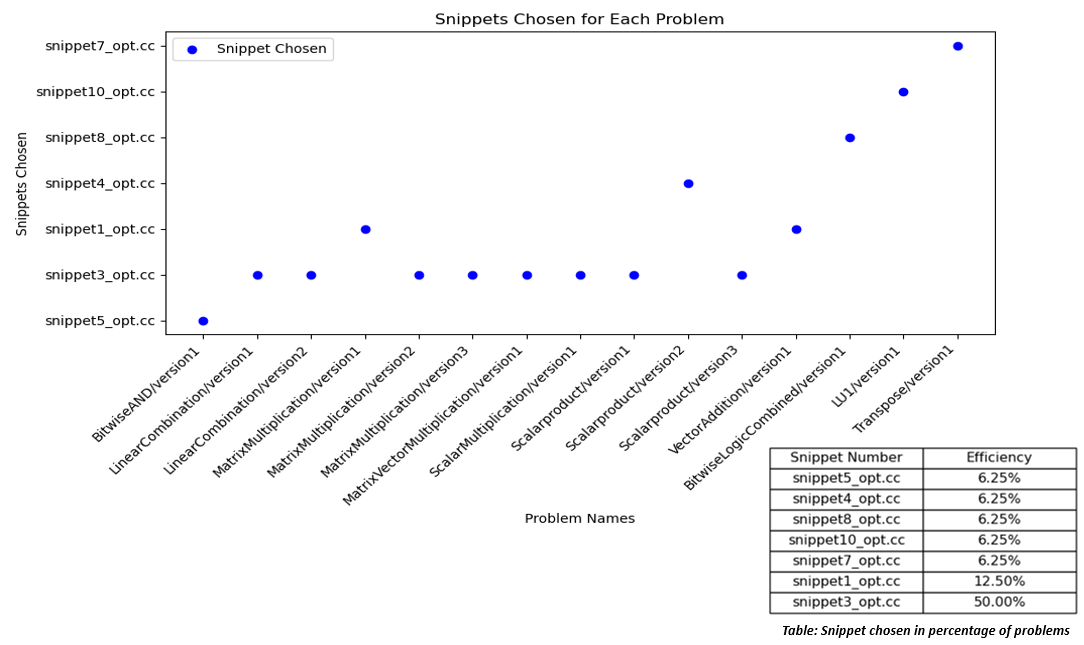
\includegraphics[height=0.8\textheight]{images/snippet-metric.png}
    \end{figure}  
\end{frame}

\begin{frame}{Architecture}
    \vspace{-1.2cm}
    \begin{figure}
        \centering
        \hspace*{1cm} 
        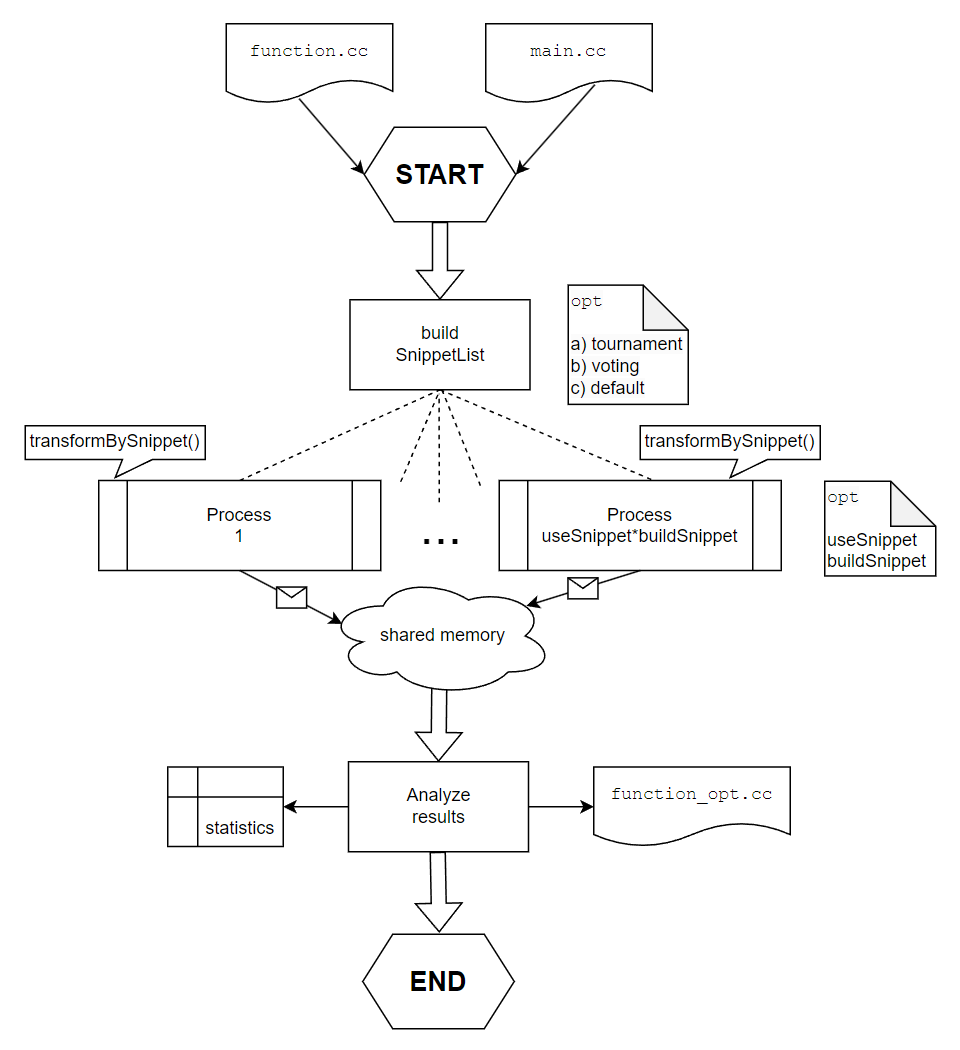
\includegraphics[height=\textheight]{images/architecture.png} 
    \end{figure}
\end{frame}

\begin{frame}{Architecture: Metrics}
    \vspace{-1.2cm}
    \begin{columns}
        \column{0.6\textwidth}
        \begin{figure}
            \centering
            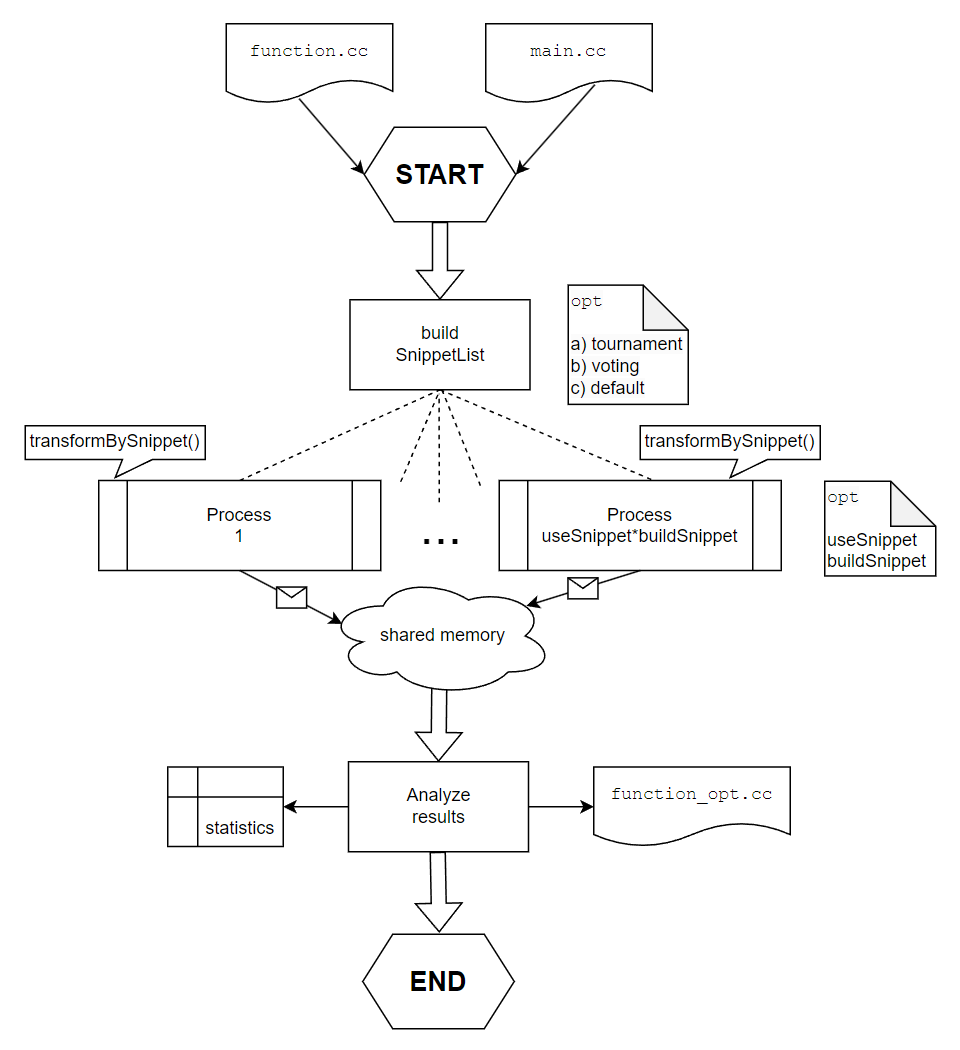
\includegraphics[height=0.8\textheight]{images/architecture.png} 
        \end{figure}
        \column{0.4\textwidth}
        \begin{tcolorbox}[width=\linewidth, colframe=CornflowerBlue]
            \centering
            \begin{tabular}{@{}lr@{}}
                \toprule
                \textbf{Type} & \textbf{LOC} \\
                \midrule
                main code & 1248 \\
                tests & 1266 \\
                \bottomrule
            \end{tabular}
        \end{tcolorbox}
    \end{columns}
\end{frame}


\begin{frame}{Project Goals: Achieved?}
    \centering
    Construct an usable AVX transformation program (\textcolor{green}{\ding{51}}\textcolor{green})
    \vfill
    \begin{table}[htbp]
        \centering
        \begin{tabular}{lc}
            \toprule
            \textbf{Task} & \textbf{Done?} \\
            \midrule
            Use meta-strategies, profiling & \textcolor{green}{\ding{51}}\textcolor{green}{\ding{51}} \\
            Prompt engineering & (\textcolor{green}{\ding{51}}) \\
            Use human feedback if necessary & (\textcolor{green}{\ding{51}}) \\
            Try model fine-tuning & \textcolor{green}{\ding{51}} \\
            Evaluate different LLMs & \textcolor{red}{\ding{55}} \\
            Implement iterative refinement & \textcolor{red}{\ding{55}} \\
            Collect examples & \textcolor{green}{\ding{51}} \\
            Implement environment for evaluation (unit tests) & \textcolor{green}{\ding{51}} \\
            Evaluate on your examples & \textcolor{green}{\ding{51}} \\
            \bottomrule
        \end{tabular}
    \end{table}
\end{frame}

\begin{frame}{Project Goals: Scope for Improvements?}
    \begin{enumerate}
        \item Transform whole programs  
        \vspace{1.0cm}
        \item Evaluate different LLMs 
        \vspace{1.0cm}
        \item Implement iterative refinement 
    \end{enumerate}
\end{frame}

\begin{frame}{Lessons Learned}
    \begin{enumerate}

        \item Choice of snippet is ambiguous
    
        \vspace{0.5cm}
        \item LLM does not possess supreme knowledge
            
        \vspace{0.5cm}
        \item Potential of Google Transform
            
        \vspace{0.5cm}    
        \item Lacking ends of ChatGPT
        
    \end{enumerate}
\end{frame}



\begin{frame}{Important Links}
    \begin{enumerate}
        
        \item Code
        \begin{itemize}
            \item \footnotesize \textcolor{magenta}{\url{https://github.com/pvs-hd-tea/23ws-PerfTuner}}
        \end{itemize}
        
        \vspace{0.3cm}
        
        \item Docs (Accounting, Developer Documentation, Video, Presentation)
        \begin{itemize}
            \item \footnotesize \textcolor{magenta}{\url{https://github.com/pvs-hd-tea/23ws-PerfTuner/tree/main/docs}}
        \end{itemize}
        
        \vspace{0.3cm}
        
        \item Data
        \begin{itemize}
            \item \footnotesize \textcolor{magenta}{\url{https://github.com/pvs-hd-tea/23ws-PerfTuner/tree/main/Product/Statistics}}
        \end{itemize}
        
        \vspace{0.3cm}
         
        \item 1-click demo
        \begin{itemize}
            \item \footnotesize \textcolor{magenta}{\url{https://github.com/pvs-hd-tea/23ws-PerfTuner/blob/main/Product/perftuner.py}}
            \item \footnotesize let it run with: \texttt{python3 perftuner.py}
        \end{itemize}
    
    \end{enumerate}
\end{frame}

\end{document}
